\documentclass[11pt]{article}
\usepackage{amsmath,amssymb}
\usepackage{graphicx}
\usepackage{array}
\usepackage{changes}
\usepackage{natbib}
\graphicspath{ {/Users/kennedy/Desktop} }
\usepackage[margin=1in]{geometry}
\usepackage[margin=1cm]{caption}
\usepackage[parfill]{parskip}  
\usepackage{gensymb}
\title{Notes on this SPAC implementation\large}
\author{Daniel Kennedy - djk2120@columbia.edu 
}

\begin{document}
\maketitle

\section{Introduction}

\clearpage
\section{Model description}

\subsection{Plant Water Supply Equations}

The basic Darcy flux is described by:

\begin{equation}
q = -\int_{\psi_{soil}}^{\psi_{leaf}}{k\left(\psi\right)d\psi}
\end{equation}

And we adopt a simple linear conductance attenuation parameterization:

\begin{equation}
k(\psi) = \dfrac{\psi - p_2}{p_1 - p_2} \cdot k_\text{max}
\end{equation}

Such that equation (1) can be rewritten as:

\begin{equation}
q = -k_\text{max}\cdot f_k\left(\Psi_L,\Psi_s\right) \cdot \left(\psi_L-\psi_s\right)
\end{equation}

Where $f_k$ is the fraction of maximal soil-to-leaf hydraulic conductance, and is a function of both $\Psi_s$ and $\Psi_L$:

\begin{equation}
f_k = \dfrac{\dfrac{1}{2} \left(\psi_L+\psi_s\right) - p_2}{p_1 - p_2} \in \left[0,1\right]
\end{equation}


\clearpage
\subsection{Plant Water Demand Equations}

Here we implement hydraulic limitations to transpiration. As $\Psi_L$ becomes more negative, transpiration is reduced relative to some maximal value, using a simple linear attenuation function. This function uses $p_3$ and $p_4$ as parameters to define the onset of transpiration reduction $p_3$ and the point at which there is no transpiration $p_4$.

\begin{equation}
T = T_\text{max}\cdot f_T
\end{equation}

\begin{equation}
f_T = \dfrac{\psi_L - p_4}{p_3 - p_4} \in \left[0,1\right]
\end{equation}

Right now we have to produce some reasonable values for $T_\text{max}$ and force the model with that data, directly. Instead we could implement a stomatal conductance model, if we would rather force with micro-met.

\begin{figure}[h]
\centering
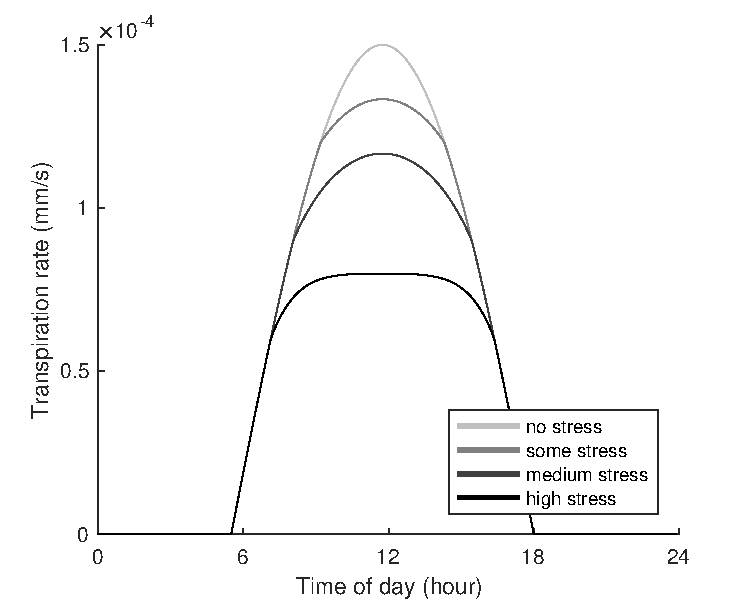
\includegraphics[width=25pc]{../figs/exp0}
\caption{We are forcing the model with the lightest gray curve. And then based on $\Psi_L$, we attenuate the transpiration accordingly. In this case, I am varying $\Psi_s$ to achieve different levels of stress.}
\label{fig:soln}
\end{figure}

\clearpage
\subsection{Solution}

We solve for leaf water potential and transpiration by requiring that: 
\begin{equation}
T = q
\end{equation}

\begin{figure}[h]
\centering
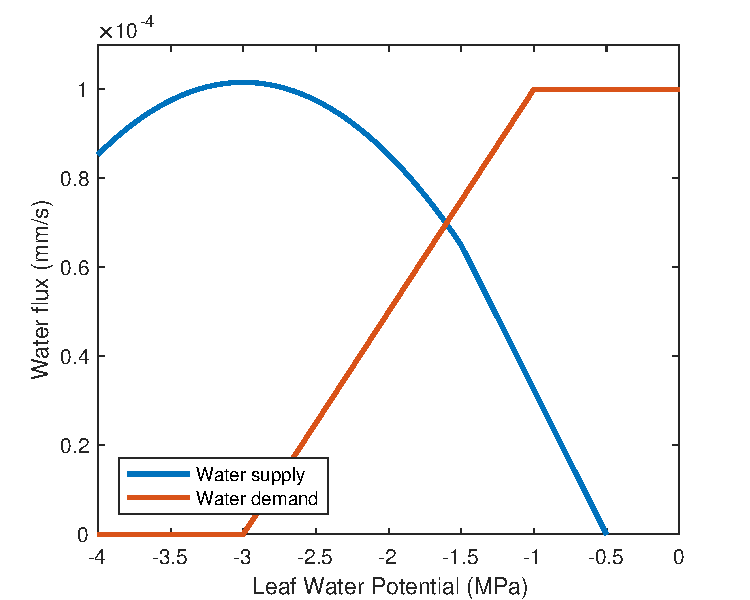
\includegraphics[width=25pc]{../figs/spac_solution}
\caption{The solution for $\Psi_L$ occurs where the two curves intersect.}
\label{fig:soln}
\end{figure}

Because transpiration decreases with decreasing $\Psi_L$ and sap flux increases, we can usually find a satisfactory solution. 

\clearpage
\subsection{Bucket}

Right now the bucket is the simplest it can be. Remove the transpiration each timestep. The bucket is sized according to the effective rooting depth $Z_r$.

\begin{equation}
\theta_1 = \theta_0 - \dfrac{q\Delta t}{Z_r}
\end{equation}

\begin{equation}
\psi_{soil}\left(\theta\right) = \psi_{soil,sat}\left(\dfrac{\theta}{\theta_{sat}}\right)^{-b}
\end{equation}

Do not currently have implementations of:
\begin{itemize}
\item Rain
\item Runoff
\item Drainage
\end{itemize}


\clearpage
\section{Experiments}

\subsection{Experiment 1}
No drainage, no rain. Looking at a 30-day drydown. I'm forcing the model with a diurnal course $T_\text{max}$, which with no stress produces approximately 4.3 mm/d of transpiration. All five runs use the same $k_\text{max}$ = 6e-5 mm/s/MPa; $Z_r$ varies from 0.5 to 2.5m.

\begin{figure}[h]
\centering
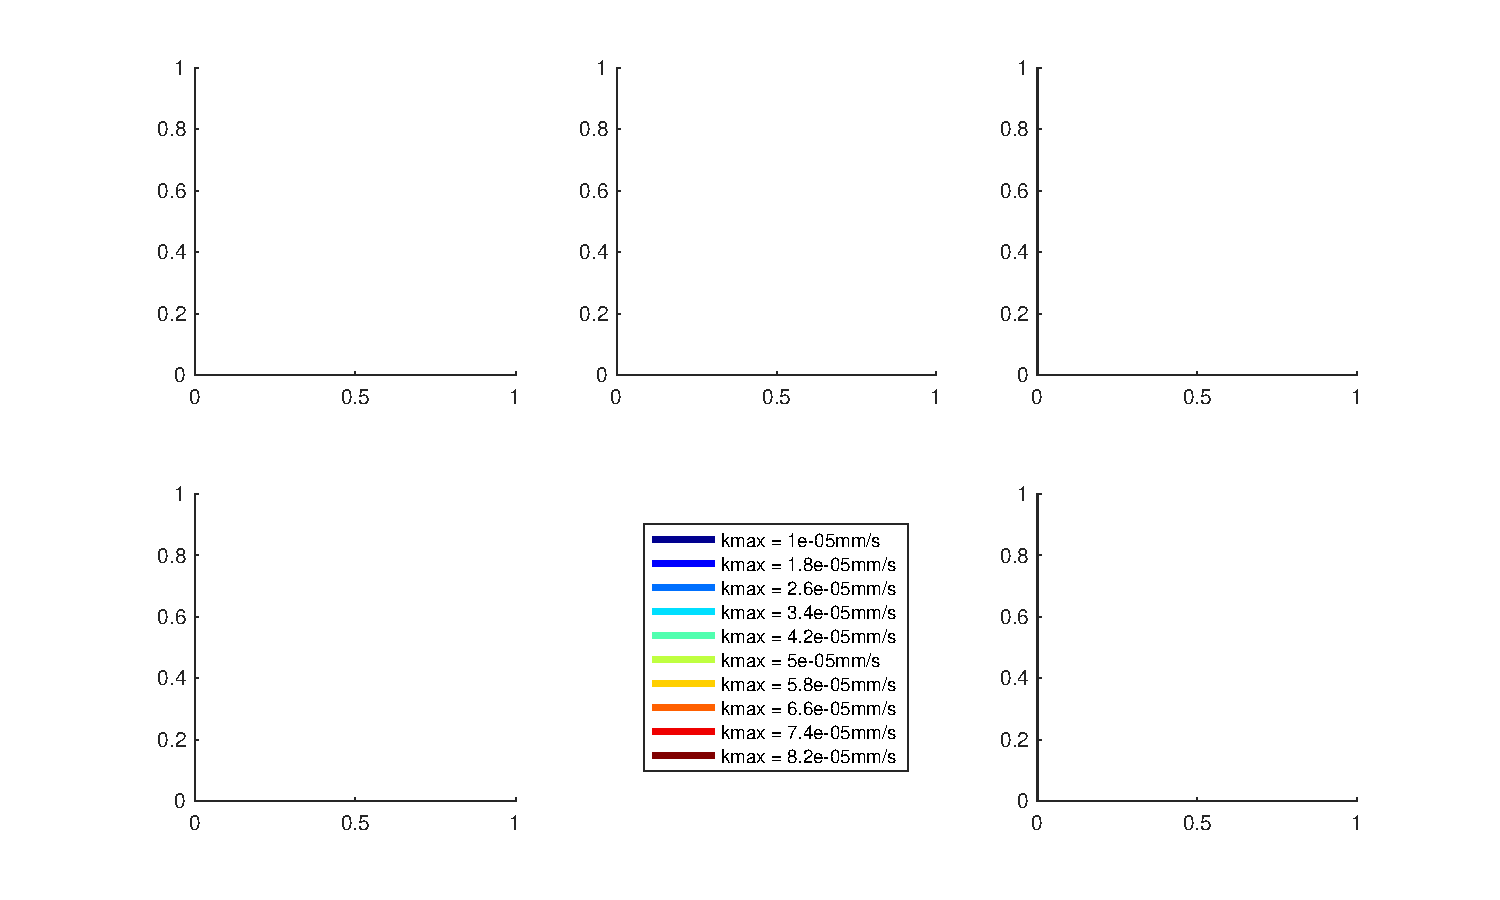
\includegraphics[width=35pc]{../figs/exp1}
\caption{Varying $Z_r$.}
\label{fig:exp1}
\end{figure}

\clearpage
\subsection{Experiment 2}
No drainage, no rain. Looking at a 30-day drydown. I'm forcing the model with a diurnal course $T_\text{max}$, which with no stress produces approximately 4.3 mm/d of transpiration. All five runs use the same $Z_r=$ 1m; $k_\text{max}$ varies from 4 to 8e-5.

\begin{itemize}
\item We should consider whether any other traits should be coordinated with $k_\text{max}$ (e.g. $p_{50}$).
\item Here a drydown doesn't seem as appropriate...
\item Maybe it's better to have some rain?
\end{itemize}


\clearpage
\subsection{Experiment 3}
Factorial approach mixing the various $Z_r$ and $k_\text{max}$.


\begin{figure}[h]
\centering
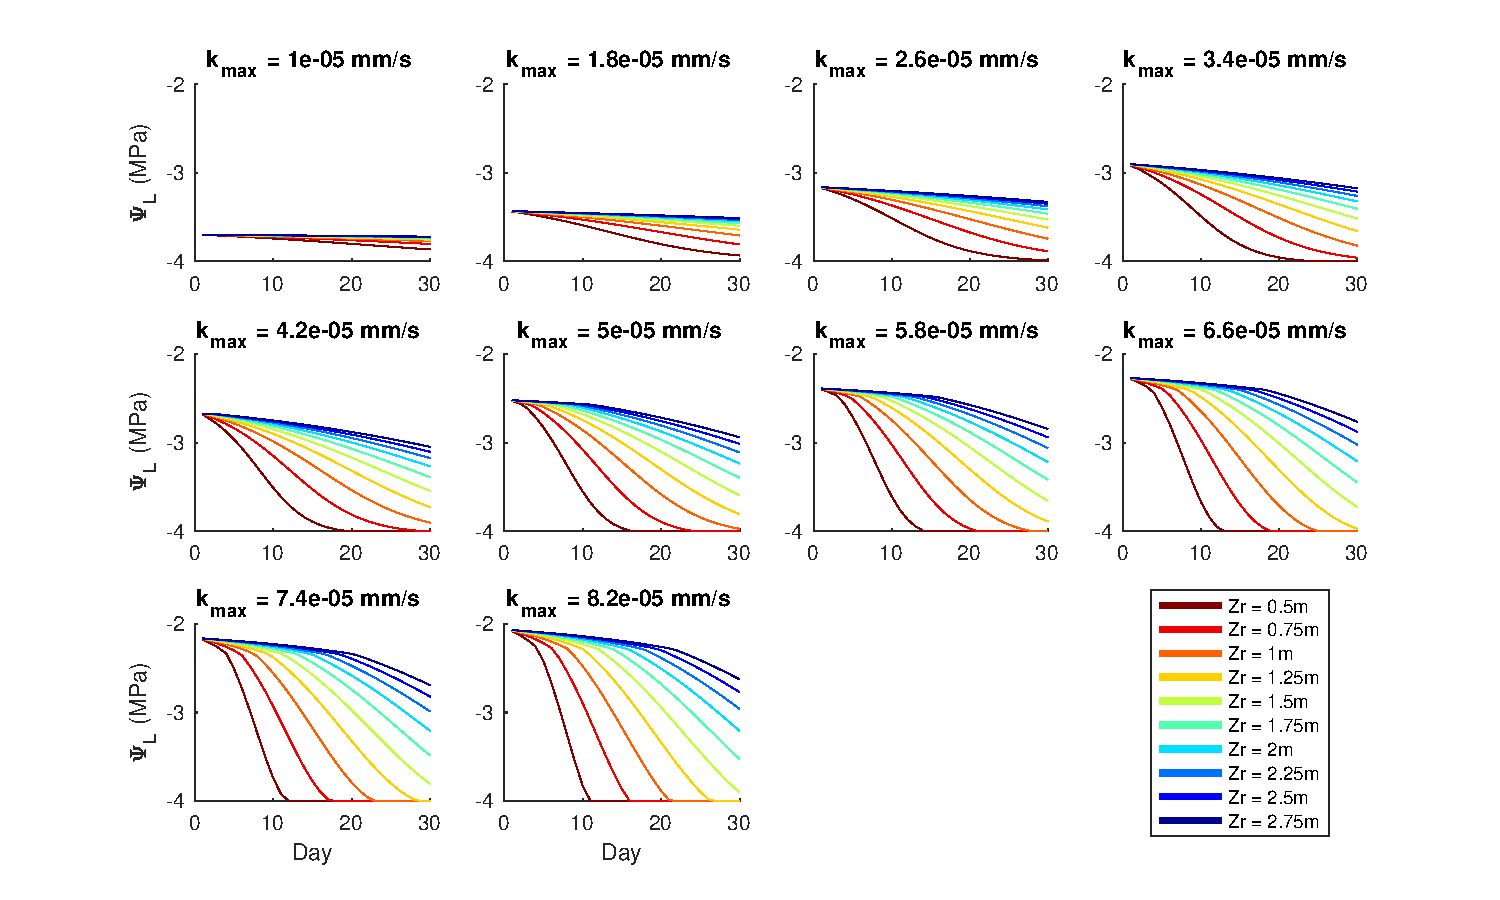
\includegraphics[width=40pc]{../figs/exp3a}
\caption{There are a couple of challenges here for retrieving the correct $Z_r$}
\label{fig:exp3a}
\end{figure}


\begin{figure}[h]
\centering
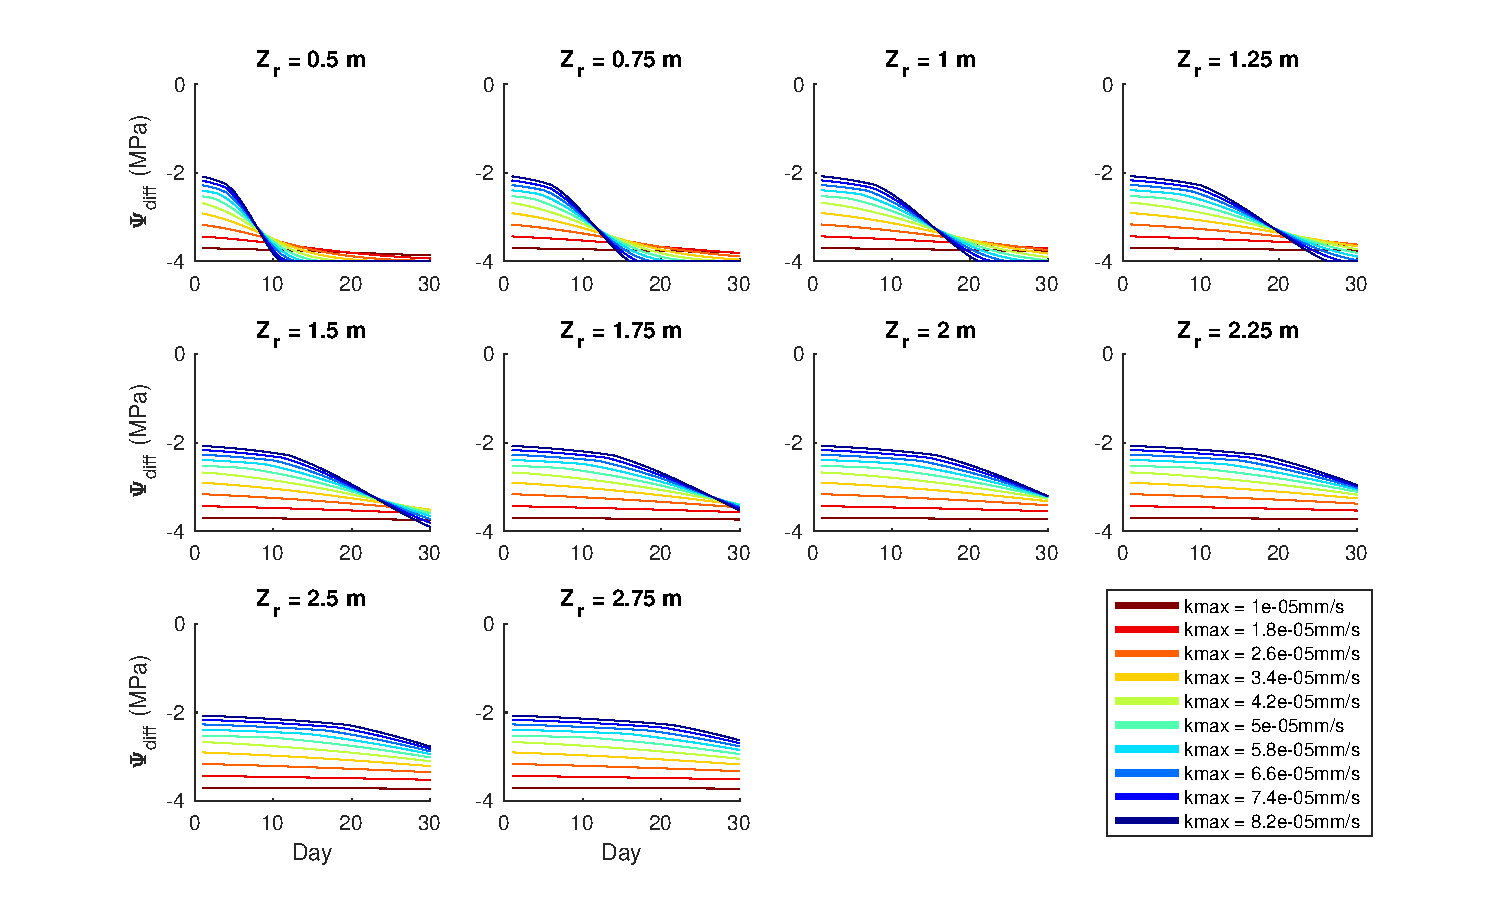
\includegraphics[width=40pc]{../figs/exp3b}
\caption{As $Z_r$ gets smaller, our classification for $k_\text{plant}$ becomes more challenging}
\label{fig:exp3b}
\end{figure}





\clearpage
\bibliographystyle{abbrvnat}
\nocite{*}

\bibliography{refs/all}





\end{document}




